\documentclass[10pt, letterpaper, twocolumn]{IEEEtran}
\usepackage{graphicx}
\usepackage{float}
\usepackage{amsmath}
\usepackage{amsfonts}
\usepackage{amssymb}
\usepackage{lipsum}
\usepackage{ctex}

\begin{document}

\title{2024年8月23日}
\author{\IEEEauthorblockN{简律纯}
\IEEEauthorblockA{}}
\maketitle

\begin{figure}[ht]
\centering
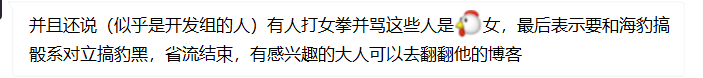
\includegraphics[width=0.8\columnwidth]{image/image1.png}
\label{fig:example}
\end{figure}

\textbf{打女拳:} 是我在空间看到的之前加的海豹用户打拳,被我忍了很久,因为火大于是就说出来了。

\textbf{妓女:} 这个确实是我说话很难听的问题,因为我想着我忍了山本多少个月的谩骂还有他们圈子的造谣,如今我破防了,我就恣无忌惮骂回去。
其实这个“夜以继日的妓女”或者“日夜赶工的妓女”是一本名著里的内容,是文艺的说法,就是说很卖力。
\marginpar{\vrule width 1pt\hspace{1pt}我有在反思了xD 不好意思。}


\textbf{骰系对立:} 对的,因为我当时不认为海豹还有什么救药了,官方的管理组都“不公平公正”,加上有很多喜欢逼着人道歉的用户似乎是社区领袖,所以搞对立(我觉得山本是要我对立的,但是他希望我对立赵)。

\begin{figure}[ht]
    \centering
    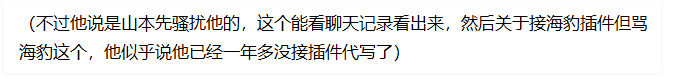
\includegraphics[width=0.8\columnwidth]{image/image2.png}
    \label{fig:example}
    \end{figure}

\end{document}

